
\section{Полетные испытания}
\subsection{Настройка полетного контроллера}
Процесс сборки квадрокоптера был описан в прошлой работе \cite{nir}, после сборки необходимо произвести конфигурацию прошивки полетного контроллера.
Последовательность действий при конфигурации системы:
\begin{itemize}
	\item Указание прошивке на тип и схему БПЛА (квадрокоптер);
	\item Калибровку датчиков (акселерометра, магнитометра, гироскопа...);
	\item Проверка корректности ориентации датчиков положения -- акселерометра и гироскопа (отклонения по всем осям происходят в нужные стороны);
	\item Конфигурация протокола радиоуправления;
	\item Калибровка и настройка каналов радиоуправления (выставлены последовательно соответствующие оси и добавлены необходимые режимы);
	\item Проверяется и задается последовательность моторов (порядковые номера моторов соответствуют используемым прошивкой полетного контроллера);
	\item Проверяется направление вращений моторов и пропеллеров (диагональные моторы вращаются в одинаковых направлениях согласно выбранной схеме ЛА).
\end{itemize}

Часто в связи с некорректной настройкой одного из описанных пунктов возникают неконтролируемые ситуации при старте -- дрон отказывается взлетать или переворачивается при взлете.

\subsection{Полетные режимы}
В прошивке реализованы различные схемы управления и стабилизации ЛА.
Такие схемы называются полетными режимами. Можно разделить на ручные и автономные.
Существуют три основных ручных полетных режима:

\begin{itemize}
	\item MANUAL;
	\item ACRO;
	\item ANGLE.
\end{itemize}

Режим MANUAL используется в основном для управления самолетом в ручном режиме, в процессе настройки и в случае непредвиденных ситуаций (отказ системы).

В режиме ACRO отклонением стиков задается угловая скорость для соответствующей  оси дрона. Центральное положение стика означает нулевую угловую скорость. В то время как угловая скорость при крайнем положении настраивается значением системы рейтов. Таким образом, при нулевом положении стика дрон не возвращается в горизонт (отсутствует стабилизация уровня). Режим ACRO используется для акробатических полетов, когда требуется плавное и быстрое управление \cite{ardupilot}. Считается самым сложным ручным режимом.

Режим ANGLE - режим стабилизации. При центральном положении стиков дрон возвращается в горизонтальное положение \cite{dcl}. Отклонение стиков пропорционально задает угол наклона дрона. Данные для регулирования берутся с акселерометра и гироскопа.

Дополнительные режимы для автопилота:
\begin{itemize}
	\item POSHOLD;
	\item ALTHOLD;
	\item OFFBOARD.
\end{itemize}

POSHOLD - удержание позиции по датчикам / компьютерному зрению.

ALTHOLD - удержание высоты по датчикам / компьютерному зрению. 

OFFBOARD — управление полетом с внешнего компьютера (например, Raspberry Pi). Этот режим используется для программирования автономных полетов \cite{clover}, при котором управление происходит из выполняемой на внешнем компьютере программы.

В ходе полетных испытаний производится полная настройка полетного контроллера и полет в ручных режимах. Это необходимо, чтобы приступить к следующей части проекта - программированию автономного полета. В случае, если ручное управление недоступно, приступать к автономным полетам нельзя -- при внештатных ситуациях (отказ оборудования, некорректное выполнение автономной миссии, сбои, преждевременное завершение задания) необходим перехват дрона в ручное управление, в противном случае возможно нанесение ущерба окружению.

Убедившись, что описанные в начале раздела пункты выполнены, был выставлен режим ACRO и проверены взлет, пролет и повороты. Далее в режиме ANGLE проверено, что после любых отклонений дрон возвращается в горизонтальное положение (рис. \ref{fig:takeoff}).

\begin{figure}[H]
	\centering
	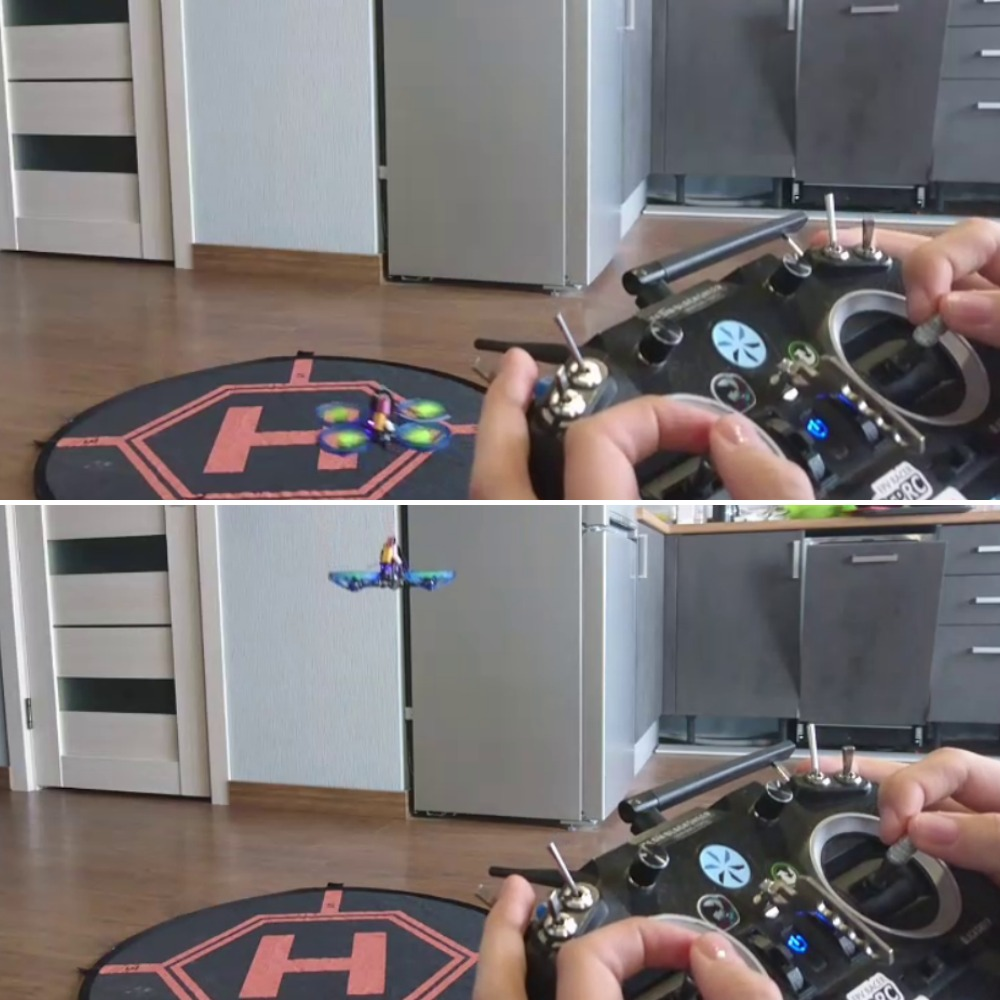
\includegraphics[width=0.5\linewidth]{pics/takeoff}
	\caption{ Первый взлет
	}
	\label{fig:takeoff}
\end{figure}

Во время полета проверяется корректная работа систем фильтрации и ПИД регулирования. Недостаточная фильтрация приведет к осцилляциям во время полета ввиду попадания шумов в ПИД регулятор. Особо чувствительной к шумам является Д-компонента. В крайних условиях излишек шумов приведет к невозможности управления и/или повреждению оборудования. После пробного полета проверяется нагрев моторов, что свидетельствует об излишке шумов.
Для объективного исследования количества шумов в системе производится логирование и анализ показаний гироскопа.

Проведенный анализ показал, что объем шумов несущественный, все гармоники находятся в области  легко фильтруемых частот (выше 120 Гц). Следующим шагом производится проверка настройки ПИД регулятора. Настройка производится стандартным методом step response \cite{tau}. Суть метода заключается в передаче ступенчатого управляющего сигнала на вход регулятора и анализе реакции системы на него.
Медленная реакция на ступенчатый управляющий сигнал указывает на низкий коэффициент пропорциональной составляющей.
Коэффициент увеличивается до появления характерного перерегулирования.
После чего остаточные осцилляции гасятся путем повышения коэффициента дифференциальной составляющей.

Таким образом, экспериментальный образец дрона доведен до финального шага -- настройки автономного полета.